\chapter{Trigonometry}%
\label{chap:trigonometry}

\section{The Pythagorean Theorem}%
\label{sec:pythagorean-thm}

Trigonometry is the study of triangles, especially \textbf{right
  triangles}. A \textbf{right triangle} is a triangle that has a
\(90^{\circ}\) angle which is often denoted by drawing a little square
in the corner where two sides meet at a perpendicular or
\(90^{\circ}\) angle.
\begin{center}
  \includestandalone{figures/right-triangle}
\end{center}

We begin our study of Trigonometry by proving three important
theorems. A \textbf{theorem} is a fact. But a theorem is more than
just a fact, it is a true statement about mathematical objects.
Mathematical objects can include a huge variety of things like shapes,
numbers, equations, inequalities, graphs, sets, plus many many more.
Usually, a theorem applies to a whole class of mathematical objects
like all triangles or all graphs.

Theorems require a \textbf{proof}, which is just a convincing
explanation of why the statement or theorem is true. It is common to
denote the end of a proof with a small square, that looks like this:
\(\square\) or \(\blacksquare\). We will present several theorems in
this book, but we won't supply a proof for each one because some of
them will require techniques or knowledge beyond the scope of our
study. Hopefully, the few we do present will give you an idea of what
a proving a theorem entails.

\begin{theorem}[Area of a Triangle]
  The area of a triangle with base, \(b\), and height, \(h\) is:
  \begin{equation}
    \label{eq:area-triangle}
    A = \tfrac{1}{2}bh
  \end{equation}
\end{theorem}
\newpage
\begin{proof}
  {~}
  \begin{center}
    \includestandalone[scale=0.75]{figures/area-triangle}
  \end{center}
  The height of the triangle divides the largest rectangle into two
  sub-rectangles. Since the triangle covers exactly half of each
  sub-rectangle, the triangle occupies exactly half of the area of the
  outer rectangle which is \(bh\).
\end{proof}

It is a common convention to use Greek letters to denote angles,
especially the letters \(\alpha\) ``alpha'', \(\beta\) ``beta'',
\(\gamma\) ``gamma'', \(\theta\) ``theta'', but sometimes Roman
letters such as x, y, z, t or capital letters such as \(A,B,C\) are
used as well.

\begin{theorem}[Sum of Interior Angles of a Triangle]
  The interior angles of a triangle sum to \(180^{\circ}\).
\end{theorem}

\begin{proof}
  {~}
  \begin{center}
    \includestandalone{figures/interior-angles-triangle-thm}
  \end{center}
  Draw a line segment between points \(a\) and \(b\) parallel to the
  base of the triangle. Extending the edges of the triangle past the
  parallel line generates angles which correspond with angles
  \(\alpha\) and \(\gamma\). Similarly, the two angles marked
  \(\beta\) are vertical angles and thus equal. Finally, the three
  angles at the top of the figure sum to a straight line and thus sum
  to \(180^{\circ}\).
\end{proof}

The next theorem is the most important one in the study of
Trigonometry.

\begin{theorem}[The Pythagorean Theorem]
  If \(a, b, c\) are lengths of the legs of a \emph{right} triangle
  where \(c\) is the \emph{hypotenuse}, then
  \begin{equation}
    \label{eq:pythagorean-thm}
    a^{2} + b^{2} = c^{2}
  \end{equation}
\end{theorem}

\begin{figure}[h]
  \begin{minipage}{0.5\linewidth}
    \centering
    \includestandalone{figures/pythagorean-thm}
  \end{minipage}%
  \begin{minipage}{0.4\linewidth}
    \caption{%
      Four exact copies of a right triangle arranged to make two squares.}%
    \label{fig:pythagorean-thm}
  \end{minipage}
\end{figure}
\begin{proof}
  First, note that the outer (partly blue shaded) quadrilateral is a
  square because each side has the same length, \(a+b\), and because
  each corner has an angle of \(90^{\circ}\). Second, note that the
  inner tilted quadrilateral is also a square because each side has
  the same length, namely \(c\), and each of its corner angles must be
  \(90^{\circ}\). This is due to the fact that the two non-right
  angles in the given right triangle must sum to \(90^{\circ}\)
  because the sum of all angles in \emph{any} triangle is
  \(180^{\circ}\). Finally, we can derive
  equation~\eqref{eq:pythagorean-thm} by equating the area of the
  whole outer square to the area of the sum of its pieces.
  \begin{align*}
    \text{Area of outer square} &= \text{Sum of the area of the pieces} \\
    (a+b)(a+b) &= c^{2} +4\left( \tfrac{1}{2} a b \right) \\
    a^{2} + \cancel{2ab} + b^{2} &= c^{2} + \cancel{2ab} \\
    a^{2} + b^{2} &= c^{2}
  \end{align*}
\end{proof}

\begin{exercise}
  Laptop computer screens are measured along the diagonal, \ie{} from
  one corner of the screen to the opposite corner. If a \US{14}{\inch}
  laptop screen is \US{8}{\inch} tall, how wide is the screen?

  \vspace*{\stretch{1}}
\end{exercise}

\begin{exercise}
  To safely use a ladder, the base of the ladder should form a
  \(75^{\circ}\) angle with level ground. A simple way to ensure this
  is to use the ``4 to 1'' rule, which says that for every
  \US{4}{\foot} of height gained you move the base \US{1}{\foot} away
  from the vertical.

  \bigskip

  \noindent What is the minimum length ladder needed to safely reach a
  roof that is \US{16}{\foot} high?

  \vspace*{\stretch{1}}
\end{exercise}

\newpage

\begin{exercise}
  A phone line would normally be installed along two consecutive edges
  of a rectangular \US{2}{\mile} by \US{4}{\mile} field. If the phone
  line costs \US{2500}[\$]{\per\mile} to install, how much will be
  saved if the phone line is installed diagonally across the field
  instead of along two of the edges?

  \vspace{3ex}
  \noindent\includestandalone{figures/field-with-phone-line}

  \vspace*{\stretch{1}}
\end{exercise}

\subsection{Converse of the Pythagorean Theorem}%
\label{sub:converse-pythagorean-thm}

A \textbf{conditional statement} is a statement of the form ``If \(P\)
then \(Q\)'' where \(P\) and \(Q\) are both sub-statements. \(P\) is
called the \textbf{hypothesis} and \(Q\) is called the
\textbf{conclusion}. For example
\begin{quotation}
  \textbf{Conditional:} If Socrates is a man, then Socrates is mortal.
  (true)
\end{quotation}
Notice that the above statement is true, that is, the conclusion is a
consequence of the hypothesis being true. We can also form three
related conditional statements (see
Table~\ref{tab:conditional-statements}). The \textbf{converse} of the
statement above, is not true:
\begin{quotation}
  \textbf{Converse:} If Socrates is mortal, then Socrates is a man.
  (false)
\end{quotation}
There are lots of things that are mortal that are not men, for example
Socrates could refer to a woman or a horse. Thus a conditional
statement and its converse need not both be true. But sometimes they
are.

\newpage

\begin{table}[h]
  \centering
  \begin{tabular}{llr@{$\:\Rightarrow\:$}l}
    \toprule
    Statement
    & English Form & \multicolumn{2}{c}{Arrow Notation} \\
    \midrule
    Conditional
    & If \(P\) then \(Q\). & \(P\) &\(Q\) \\
    Converse
    & If \(Q\) then \(P\). & \(Q\) &\(P\) \\
    Inverse
    & If not \(P\) then not \(Q\). & \(\neg P\) &\(\neg Q\) \\
    Contrapositive
    & If not \(Q\) then not \(P\). & \(\neg Q\) &\(\neg P\)\\
    \bottomrule
  \end{tabular}
  \caption{Four types of conditional statements}%
  \label{tab:conditional-statements}
\end{table}

The Pythagorean theorem is a \textbf{conditional statement} of the
form ``If \(P\) then \(Q\)'', where (after removing details) we
essentially have:
\begin{quotation}
  \textbf{Pythagorean Theorem:} If right triangle, then
  \(a^{2}+b^{2} = c^{2}\).
\end{quotation}
The converse of the Pythagorean theorem is of the form ``If \(Q\),
then \(P\)'', that is,
\begin{quotation}
  \textbf{Converse of Pythagorean Theorem:} If \(a^{2}+b^{2} = c^{2}\),
  then right triangle.
\end{quotation}
It turns out that the converse of the Pythagorean theorem is also
true.

\begin{theorem}[Converse of the Pythagorean Theorem]
  If \(a,b,c\) are sides of a triangle with \(c\) the longest side and
  \(a^{2} + b^{2} = c^{2}\), then the triangle is a \emph{right}
  triangle.
\end{theorem}
\begin{proof}
See appendix~\ref{app:converse-pythagorean-thm}.
\end{proof}

\begin{exercise}
  Use the converse of the Pythagorean theorem to prove that a
  triangle with sides (5,12,13) is a right triangle.

  \vspace*{\stretch{1}}
\end{exercise}

When both a conditional and its converse are always true we call it a
\textbf{biconditional}. This means that \(P\) implies \(Q\) but also
\(Q\) implies \(P\), in arrow notation: \(P \Leftrightarrow Q\). In
other words, statements \(P\) and \(Q\) are different but they both
mean the same thing. One side of the Pythagorean theorem is about
lengths and the other is about angles. And what it means is that (in
the context of triangles), knowing something about lengths of the legs
tells you something about the interior angles and vice versa. You can
think of it as a \emph{bridge} between the concept of length and the
concept of angle. This bridge leads to two new concepts: Pythagorean
triples and a way to classify triangles.

\newpage

\subsection{Pythagorean Triples}%
\label{sub:pythagorean-triples}

\begin{definition}
  A \textbf{Pythagorean triple} is any triple of whole numbers,
  \((a,b,c)\), which satisfy \(a^{2} + b^{2} = c^{2}\) and thus are
  the legs of a right triangle.
\end{definition}

\begin{example}
  Some examples of Pythagorean triples are:
  \[
    (3,4,5), (6,8,10), (5,12,13), (7,24,25), (9,40,41)
  \]
  These are useful to remember mostly because Math teachers like to
  use them in homework problems and tests, and it can save you time if
  you notice that you are dealing with one of these special triangles.
\end{example}

\begin{exercise}
  Can you take any Pythagorean triple and generate a new triple just
  by multiplying every number by a whole number, like 2 or 3? Can you
  prove it?

  \vspace*{\stretch{1}}
\end{exercise}

\newpage

\subsection{Classification of Triangles}%
\label{sub:classification-triangles}

The converse of the Pythagorean theorem allows us to use the sides of
a triangle to determine something about one of the angles. If we
combine this fact with the fact that all of the interior angles of a
triangle must sum to \(180^{\circ}\), then we can classify triangles
into three categories.

\begin{definition}
  \begin{description}
  \item[obtuse angle: ] an angle between \(90^{\circ}\) and \(180^{\circ}\).
  \item[acute angle: ] an angle between \(0^{\circ}\) and \(90^{\circ}\).
  % \item[right angle: ] an angle that is exactly \(90^{\circ}\).
  \item[obtuse triangle: ] a triangle which has one obtuse angle.
  \item[acute triangle: ] a triangle where all angles are acute.
  % \item[right triangle: ] a triangle which has one right angle.
  \end{description}
\end{definition}

\begin{table}[h]
  \centering
  \begin{tabular}{m{3cm}m{4cm}m{2cm}}
    \toprule
    Condition
    & Example
    & Category \\
    \midrule
    \(c^{2} > a^{2}+b^{2}\)
    & \includestandalone[scale=0.75]{figures/small-obtuse}
    & obtuse \\
    \(c^{2} = a^{2}+b^{2}\)
    & \includestandalone[scale=0.75]{figures/small-right}
    & right \\
    \(c^{2} < a^{2}+b^{2}\)
    & \includestandalone[scale=0.75]{figures/small-acute}
    & acute \\
    \bottomrule
  \end{tabular}
  \caption{Classification of triangles by sides}%
  \label{tab:classification-triangles}
\end{table}

\begin{exercise}
  Classify the triangles with sides \((5,6,7)\) and \((5,6,8)\).

  \vspace*{\stretch{1}}
\end{exercise}

% \think{The way experienced carpenters and masons guarantee a
%   rectangular shape is first they make sure that both pairs of
%   opposite sides are of equal length, and then they measure both
%   diagonals and ensure they are equal lengths. Why does this guarantee
%   a rectangle?}

\newpage

\subsection{The Distance Formula}%
\label{sub:distance-formula}

We can use the Pythagorean theorem to find the distance between any
two points in the Cartesian plane. The basic idea is to construct a
right triangle with hypotenuse corresponding to a segment between the
two points and one leg parallel to the \(x\)-axis and another leg
parallel to the \(y\)-axis.

\begin{figure}[h]
  \centering
  \begin{minipage}{0.45\linewidth}
    \includestandalone{figures/distance-formula-1}
  \end{minipage}%
  \(\myOutlineRightArrow\)
  \begin{minipage}{0.45\linewidth}
    \includestandalone{figures/distance-formula-2}
  \end{minipage}
  \caption{The Pythagorean theorem can be used to determine distance
    bewteen points.}\label{fig:distance-formula}
\end{figure}

\begin{align}
  d^{2} &= {(x_2-x_1)}^{2} + {(y_2-y_1)}^{2} \nonumber \\
  \Aboxed{d &= \sqrt{{(x_2-x_1)}^{2} + {(y_2-y_1)}^{2}}} \label{eq:distance-formula}
\end{align}

\begin{exercise}
  Find the distance between the points \((-1,5)\) and \((2,-2)\).

  \vspace*{\stretch{1}}
\end{exercise}

\dnote{Formula~\eqref{eq:distance-formula} can be hard to remember. I
  find it easier to just remember the idea of equating the distance to
  the hypotenuse and then using a sketch and the Pythagorean theorem
  to compute the distance. }

\newpage

\section{Trigonometric Functions}%
\label{sec:trigonometric-functions}

The Pythagorean theorem allows us to determine the length of an
unknown side of a right triangle when we know two of the other sides.
But in some circumstances, we may only know an interior angle and a
side. In this section we will define six functions that will allow us
to determine sides when we only know a side and an angle.

In order to define these functions we use three terms to identify the
edges or legs of the triangle: \textbf{hypoteneuse},
\textbf{opposite}, and \textbf{adjacent}. First, the term
\textbf{hypotenuse} always refers to the longest edge of the triangle.
Next, we have the side \textbf{opposite} the angle of interest, say
\(\theta\). Finally, we have the side \textbf{adjacent} to the angle
of interest. Figure~\ref{fig:opp-adj-hyp} demonstrates how the
adjacent and opposite sides switch depending on where \(\theta\) is.
\begin{figure}[h]
  \centering
  \includestandalone{figures/opp-adj-hyp}
  \caption{Opposite and adjacent sides depend on where \(\theta\) is
    located.}%
  \label{fig:opp-adj-hyp}
\end{figure}

\subsection{The Sine, Cosine, and Tangent Functions}%
\label{sub:sin-cos-tan}

\begin{definition}
  Given a \emph{right} triangle with angle \(\theta\), we define three
  functions in terms of ratios of the sides of the triangle.
  \begin{equation}
    \label{eq:sin-cos-tan}
    \sin(\theta) = \frac{\text{opp}}{\text{hyp}} \qquad
    \cos(\theta) = \frac{\text{adj}}{\text{hyp}} \qquad
    \tan(\theta) = \frac{\text{opp}}{\text{adj}}
  \end{equation}
  A mnemonic for remembering all three definitions is SOH-CAH-TOA.
\end{definition}

\begin{example}
  Use the triangle below to compute: \(\sin(\theta), \cos(\theta)\)
  and \(\tan(\theta)\).

  \includestandalone{figures/5-12-13}

\end{example}
\begin{solution}
  \[
    \sin(\theta) = \frac{5}{13} \qquad
    \cos(\theta) = \frac{12}{13} \qquad
    \tan(\theta) = \frac{5}{12}
  \]
\end{solution}

\newpage

The three trigonometric functions we just defined are \textbf{side
  finders}. Later we will introduce functions that are \textbf{angle
  finders}.

\dnote{Make sure your calculator is in \emph{degrees} mode and not
  radians mode.}

\begin{exercise}
  Find \(x\).

  \includestandalone{figures/find-side-cos}

  \vspace*{\stretch{1}}
\end{exercise}

\begin{exercise}
  Find \(y\).

  \includestandalone{figures/find-side-sin}

  \vspace*{\stretch{1}}
\end{exercise}

\begin{exercise}
  Find \(x\).

  \includestandalone{figures/find-side-tan}

  \vspace*{\stretch{2}}
\end{exercise}

\newpage

\subsection{Inverse Trigonometric Functions}%
\label{sub:inverse-trigonometric-functions}

Not all functions have an inverse, but the three trigonometric
functions we just defined do! Recall that a function is a mapping
between two sets which we call the domain and codomain. The
\textbf{domain} of a function is the set of acceptable inputs, while a
function's \textbf{codomain} is its output set.

An inverse function maps in the reverse direction, so it swaps the
domain and codomain sets. Thus while the three trigonometric functions
eat angles and output ratios, the three \emph{inverse} trigonometric
functions eat ratios and output angles. You should think of them as
\textbf{angle finders}.

Since we have defined the three trigonometric functions via
\emph{right} triangles only, the domains and codomains are somewhat
restricted. If you take a full course on Trigonometry, you will learn
how these functions can be extended to larger domains and codomains.

\begin{table}[h]
  \centering
  \begin{tabular}{r@{ : }c@{ \(\mapsto\) }lr@{ : }c@{ \(\mapsto\) }l}
    \toprule
    Function
    & Domain
    & Codomain
    & Inverse
    & Domain
    & Codomain \\
    \midrule
    \(\sin(x)\)
    & \([0^{\circ}, 90^{\circ}]\)
    & \([0,1]\)
    & \(\sin^{-1}(x)\)
    & \([0,1]\)
    & \([0^{\circ}, 90^{\circ}]\) \\
    \(\cos(x)\)
    & \([0^{\circ}, 90^{\circ}]\)
    & \([0,1]\)
    & \(\cos^{-1}(x)\)
    & \([0,1]\)
    & \([0^{\circ}, 90^{\circ}]\) \\
    \(\tan(x)\)
    & \([0^{\circ}, 90^{\circ})\)
    & \([0,\infty)\)
    & \(\tan^{-1}(x)\)
    & \([0,\infty)\)
    & \([0^{\circ}, 90^{\circ})\) \\
    \bottomrule
  \end{tabular}
  \caption{The three Trigonometric functions map angles to ratios,
    while their inverses map ratios to angles.}%
  \label{tab:domain-range-trig-funcs}
\end{table}

\begin{exercise}
  Find \(\theta\).

  \includestandalone{figures/find-theta-sin}

  \vspace*{\stretch{1}}
\end{exercise}

\begin{exercise}
  Find \(\theta\).

  \includestandalone{figures/find-theta-tan}

  \vspace*{\stretch{1}}
\end{exercise}

\newpage

\begin{exercise}
  A new \US{500}{\foot} long zip line is going to be installed at
  Lagoon. The zip line will have a vertical distance of \US{200}{\foot}.
  At what angle will the zip line meet the ground? What is the
  horizontal distance of the zip line?

  \vspace*{\stretch{1}}
\end{exercise}

\subsection{Finding the Area of a Triangle}%
\label{sub:area-triangle}

\begin{exercise}
  Find the area of the given triangle using trigonometric functions.

  \vspace*{\stretch{1}}
\end{exercise}

\newpage

\subsection{Angles of Elevation and Depression}%
\label{sub:angles-elevation-depression}

\begin{exercise}
  A person stands \US{300}{\foot} from the base of a cliff. The angle
  of elevation to the bottom of a tree atop the cliff is
  \(40^{\circ}\). The angle of elevation to the top of the tree is
  \(43^{\circ}\). How tall is the tree?

  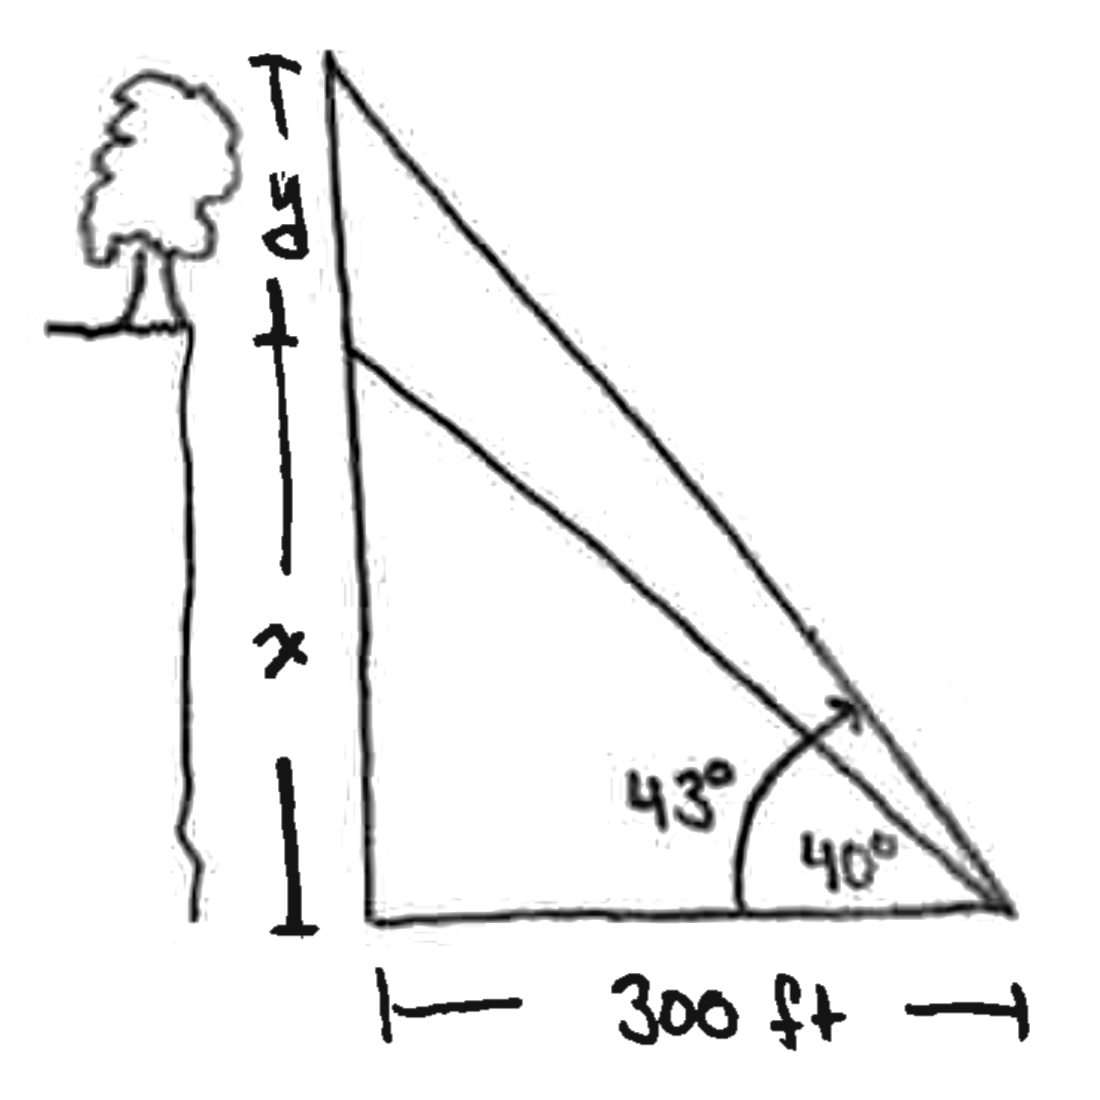
\includegraphics[scale=0.15]{tree-on-hill}

  \vspace*{\stretch{1}}
\end{exercise}

\begin{exercise}
  A statue is located \US{300}{\foot} from a building. From a window
  in the building, a person determines that the angle of elevation to
  the top of the statue is \(34^{\circ}\) and the angle of depression
  to the bottom of the statue is \(22^{\circ}\). How tall is the
  statue?

  \vspace*{\stretch{2}}
\end{exercise}

\dnote{Beware the functions we define in this section only apply to
  \emph{right} triangles.}



%%% Local Variables:
%%% mode: latex
%%% eval: (outline-minor-mode 1)
%%% TeX-master: "Notes"
%%% End:
